\documentclass{article}

\usepackage{amsmath}
\usepackage{amssymb}
\usepackage{graphicx}
\usepackage{hyperref}
\usepackage{xcolor}
\usepackage{listings}
\graphicspath{ {images/} }
\setlength\parindent{0pt}

\lstset{frame=tb,
	language=C++,
  	aboveskip=4mm,
  	belowskip=12mm,
  	showstringspaces=false,
  	columns=flexible,
  	basicstyle={\small\ttfamily},
  	numbers=none,
  	numberstyle=\tiny\color{gray},
  	keywordstyle=\color{blue},
  	commentstyle=\color{brown},
  	stringstyle=\color{mauve},
  	breaklines=true,
  	breakatwhitespace=true,
  	tabsize=4
}


\title{
	\Huge
	{Building a 3-D Physics Engine to Model Projectile Motion}\\
}
\author{Maxim Webb}

\begin{document}

\maketitle

\newpage

\begin{abstract}
In this report, I will describe the process of building a 3-D physics engine, with the end goal being to create an accurate model for projectile motion.
\newline
\newline
However, this is not the sole goal; the aim throughout the project is to build a physics engine from first principles, without relying on pre-existing 3-D graphical APIs such as OpenGL, or Direct3D. Therefore, the report will also describe the mathematics behind the rendering process, as well as the necessary methods for representing 3-D transformations.
\newline
\end{abstract}
\newpage
\tableofcontents

\newpage

\section{Technology}
The program will be written in C++, for its speed, and for its object orientation, which will prove useful for the structure of the project. This includes the use of several template classes from the STL, such as \verb|<cmath>| and \verb|<vector>|.
\newline
\newline
Windows GDI will be used for basic graphical output, which is limited to drawing lines and polygons. 
\newline
\newline
Git will be used for this project, providing versatile and powerful VCS. The project's source code is available 
\href{https://github.com/maximwebb/3D-engine}{\color{blue} on Github}\color{black}.

\newpage
\section{Basic Structure}

First, the Point class will be the building blocks of engine, with the parameter \verb|abs_pos| describing the absolute position in the universe. The declared methods \verb|update()| and \verb|draw()| will be fleshed out later.
\begin{lstlisting}
class Point {
public:
	/* Parameters */
	vector<float> abs_pos;
	
	void update() {
	
	}
	
	void draw(HDC hdc) {
	
	}
}
\end{lstlisting}

Next, the Plane class stores an array of points, and contains a method for updating them, as well as a method for drawing the plane itself. 
\begin{lstlisting}
class Plane {
public:
	/* Parameters */
	vector<Point> points;
	
	void update_points() {
		for (int p = 0; p < points.size(); p++) {
			points[p].update();
		}
	}
	
	void fill_plane(HDC hdc) {
	
	}
}
\end{lstlisting}
\newpage
The Obloid class is the umbrella class for all 3-D objects in the program. Obloids will take four points as parameters, and generate the remaining four vertices. From this, six planes (faces) can be constructed, and stored in an array. 
\newline
\newline
Obloids will also store physical attributes, such as mass and velocity, which will be added later.

\begin{lstlisting}
class Obloid {
public:

	/* Parameters: Top-Right-Front, Top-Right-Back, Bottom-Left-Back, Bottom-Left-Front */
	Point trf{ { 0, 0, 0, 1 } };
	Point trb{ { 0, 0, 0, 1 } };
	Point blb{ { 0, 0, 0, 1 } };
	Point blf{ { 0, 0, 0, 1 } };
	
	/* Generate remaining four vertices */
	Point brf{ { blb.abs_pos[0], trf.abs_pos[1], trf.abs_pos[2], 1 } };
	Point brb{ { blb.abs_pos[0], trf.abs_pos[1], blb.abs_pos[2], 1 } };
	Point tlf{ { trf.abs_pos[0], blb.abs_pos[1], trf.abs_pos[2], 1 } };
	Point tlb{ { trf.abs_pos[0], blb.abs_pos[1], blb.abs_pos[2], 1 } };
	
	/* Generate six planes */	
	Plane pl_top{ { trf, trb, tlb, tlf } };
	Plane pl_bottom{ { brf, brb, blb, blf } };
	Plane pl_left{ { tlf, tlb, blb, blf } };
	Plane pl_right{ { trf, brf, brb, trb } };
	Plane pl_front{ { trf, tlf, blf, brf } };
	Plane pl_back{ { trb, tlb, blb, brb } };
	
	vector<Plane> faces = { pl_left, pl_right, pl_bottom, pl_top, pl_back, pl_front };
	
	void update_faces(HDC hdc) {
		for (int f = 0; f < faces.size(); f++) {
			faces[f].update_points(hdc);
			faces[f].fill_plane(hdc);
		}
	}
}
\end{lstlisting}

There will also be a Player class created later, in order to store information about the viewer, such as the angle and the velocity. 
\newpage

\section{Projecting onto the viewport}
When considering displaying objects on the viewport (the visible section of the screen), it becomes evident that a method is required for converting between the 3-D coordinates of the universe, and the 2-D coordinates of the viewport. This process must account for depth, thereby providing perspective.

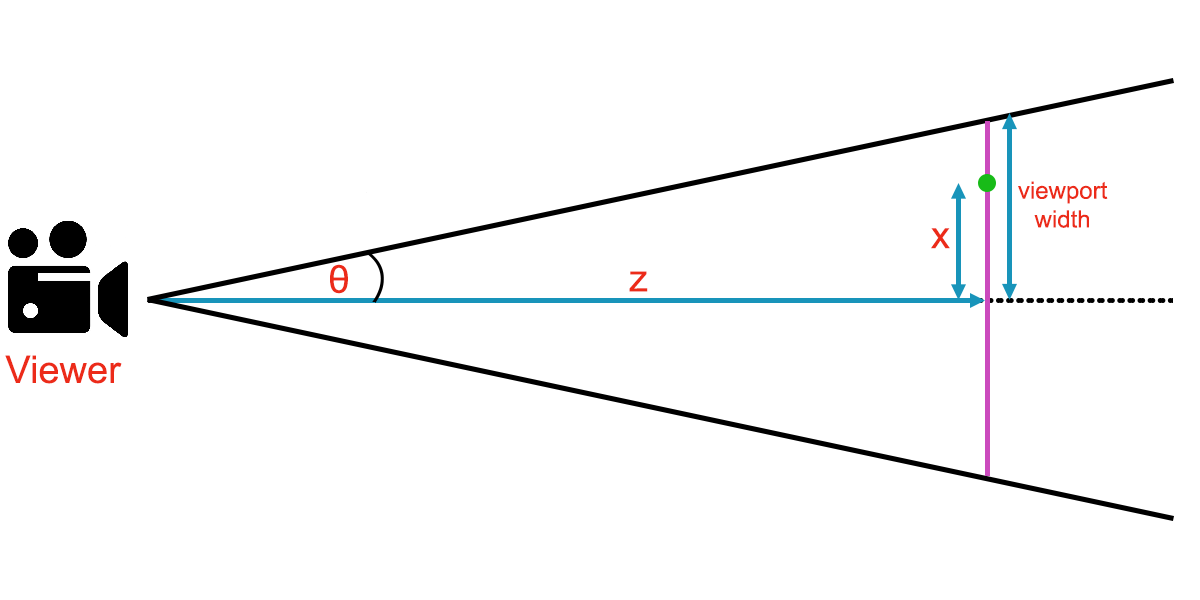
\includegraphics[width=1\textwidth]{projection_diagram.png}

The diagram shows a bird's eye view of the viewer's vision. The green dot represents a point in the viewer's line of sight, and is a certain z-distance away from the viewer. At this z-distance, there is a virtual plane to project the point onto, represented by the pink line. 
\newline
\newline
Then, the width of the virtual plane, and the ratio of this width to the point's displacement from the centre line is found as follows:
\newline
\newline
Let p = plane width, let x, z be coordinates of point:
$$ p = ztan{\theta} $$
$$ ratio = \frac{x}{ztan{\theta}} $$
Applying the same logic, the vertical ratio is $ \frac{y}{ztan{\theta}} $
\newline
\newline
Then, if the screen has width w and height h, the coordinates on the window $(s_x, s_y) $ are as follows:

$$ s_x = \frac{1}{2}w + \frac{xw}{ztan{\theta}} $$
$$ s_y = \frac{1}{2}h + \frac{yh}{ztan{\theta}} $$
\newpage
It is worth noting at this point that this method only works if the viewer is centred about (0, 0, 0). Therefore, in the Point class definition, there should be a second position coordinate, relative to the viewer. With this new type of coordinate, \verb|update()| can now be defined as shown:

\begin{lstlisting}
class Point {
public:
	/* Parameters */
	vector<float> abs_pos;
	
	vector<float> rel_pos;
	int screen_x;
	int screen_y;	
	
	void update() {
		screen_x = window_width * 0.5 + window_width * rel_pos[0] / (rel_pos[2] * tan(fov));

		screen_y = window_height * 0.5 + window_width * rel_pos[1] / (rel_pos[2] * tan(fov));
	}
	
	void draw(HDC hdc) {
	
	}
}

\end{lstlisting}
For clarity's sake, some of the variables have been renamed in the code, but the function is the same as the previous result.

\newpage

\section{Transformations of 3-D space}
Now that projections onto the viewport has been implemented, there needs to be a way of the viewer moving around the universe. This requires translating and rotating the universe about the viewer.
\newline
\newline
There are several methods for handling these transformations - one approach would be the use of quaternions, which are an extension of complex numbers, 

\end{document}